\chapter*{Výsledky}
\par Pro účely demonstrace implementovaného algoritmu \emph{Partial Modification} pro modifikaci jednoho prvku byly z databáze ArcČR 500 3.3 obdrženy dvě linie – silnice (černá barva) a vodní tok (modrá barva) v blízkosti Špindlerova Mlýnu (viz. Obrázek 2). Při zachování výchozích parametrů:
\begin{itemize}
    \item[] \underbar{$d$} = 100 m,
    \item[] počet iterací $50$,
    \item[] $\alpha = 1,$
    \item[] $\beta = 1000,$
    \item[] $\gamma = 10,$
    \item[] $\lambda = 10$
\end{itemize}
\par byl proveden odsun silnice (červená barva) na místech, kde do sebe obě linie splývají, což je znázorněno na Obrázku 4. S tímto nastavením zachovává nová linie původní tvar silnice.
\begin{figure}[H]
\centering
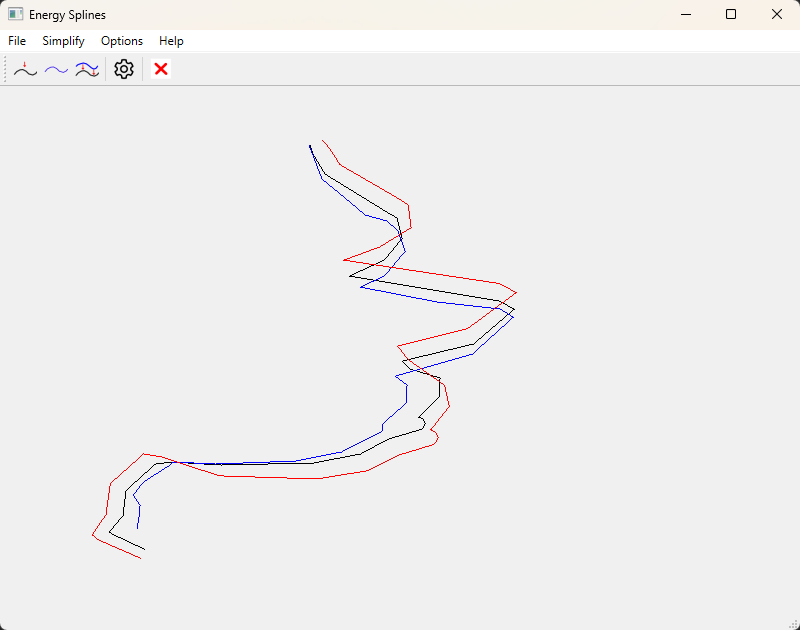
\includegraphics[width=14cm]{images/displacement.png} 
    \caption{Odsun liniového prvku s výchozím nastavením.}
\end{figure}
